\documentclass[12pt,letterpaper]{article}
\usepackage{graphicx,textcomp}
\usepackage{natbib}
\usepackage{setspace}
\usepackage{fullpage}
\usepackage{color}
\usepackage[reqno]{amsmath}
\usepackage{amsthm}
\usepackage{fancyvrb}
\usepackage{amssymb,enumerate}
\usepackage[all]{xy}
\usepackage{endnotes}
\usepackage{lscape}
\newtheorem{com}{Comment}
\usepackage{float}
\usepackage{hyperref}
\newtheorem{lem} {Lemma}
\newtheorem{prop}{Proposition}
\newtheorem{thm}{Theorem}
\newtheorem{defn}{Definition}
\newtheorem{cor}{Corollary}
\newtheorem{obs}{Observation}
\usepackage[compact]{titlesec}
\usepackage{dcolumn}
\usepackage{tikz}
\usetikzlibrary{arrows}
\usepackage{multirow}
\usepackage{xcolor}
\newcolumntype{.}{D{.}{.}{-1}}
\newcolumntype{d}[1]{D{.}{.}{#1}}
\definecolor{light-gray}{gray}{0.65}
\usepackage{url}
\usepackage{listings}
\usepackage{color}

\definecolor{codegreen}{rgb}{0,0.6,0}
\definecolor{codegray}{rgb}{0.5,0.5,0.5}
\definecolor{codepurple}{rgb}{0.58,0,0.82}
\definecolor{backcolour}{rgb}{0.95,0.95,0.92}

\lstdefinestyle{mystyle}{
	backgroundcolor=\color{backcolour},   
	commentstyle=\color{codegreen},
	keywordstyle=\color{magenta},
	numberstyle=\tiny\color{codegray},
	stringstyle=\color{codepurple},
	basicstyle=\footnotesize,
	breakatwhitespace=false,         
	breaklines=true,                 
	captionpos=b,                    
	keepspaces=true,                 
	numbers=left,                    
	numbersep=5pt,                  
	showspaces=false,                
	showstringspaces=false,
	showtabs=false,                  
	tabsize=2
}
\lstset{style=mystyle}
\newcommand{\Sref}[1]{Section~\ref{#1}}
\newtheorem{hyp}{Hypothesis}

\title{Problem Set 1}
\date{Due: January 28, 2026}
\author{Data Visualisation for Social Scientists}

\begin{document}
	\maketitle
	
	\section*{Instructions}
	\begin{itemize}
	\item Please show your work! You may lose points by simply writing in the answer. If the problem requires you to execute commands in \texttt{R}, please include the code you used to get your answers. Please also include the \texttt{.R} file that contains your code. If you are not sure if work needs to be shown for a particular problem, please ask.
\item Your homework should be submitted electronically on GitHub.
\item This problem set is due before 23:59 on Wednesday January 28, 2026. No late assignments will be accepted.
	\end{itemize}
	
	\vspace{1cm}
	\section*{Roll Call Votes in the European Parliament}

\subsection*{Data Manipulation}
First, you need to \href{https://personal.lse.ac.uk/hix/HixNouryRolandEPdata.HTM}{download data} from the first six elected European Parliaments on each MEP and how they voted in each recorded roll-call vote.

\vspace{.25cm}

\begin{enumerate}
\item Load these datasets into your global environment:
\begin{itemize}
	\item \texttt{mep\_info\_26Jul11.xls} (MEP characteristics, EP1–EP5)
	\item \texttt{rcv\_ep1.txt} (EP1 roll-call votes)
\end{itemize}
\lstinputlisting[language=R, firstline=12, lastline=13]{PS01.R}  
\item Briefly describe (2–3 sentences each) the unit of analysis and key variables in each of these two datasets.
\begin{description}
	\item The unit analysis for the EP 1 dataset is the way of which each MEP voted. The key variables are MEP ID, Vote, Vote ID, and Country. The unit of analysis for the MEP dataset is each MEP in the term. The key variables are MEP ID, EPG, National Party, NOM D1, NOM D2, and country. This dataset is more of the attributes of the MEP while the EP 1 is more focused on the vote preference of each MEP. 
\end{description}

\item The \texttt{rcv\_ep1} data are in a wide format, with V1, V2, …, Vn as separate vote columns.
\begin{itemize}
	\item Identify which columns are ID/metadata (\textit{MEPID, MEPNAME, MS, NP, EPG}) and which columns are vote decisions ($V_1$…$V_n$). Tidy the voting data such that each row/observation is a single vote for a single MEP.
	\item Create a summary table of counts of decision categories (e.g. Yes/No/Abstain/Present but did not vote/Absent) across all votes.
\lstinputlisting[language=R, firstline=17, lastline=40]{PS01.R}  
\begin{description}
	\item For this section of manipulation, I converted the EP 1 data into a long format so I could have access to every vote outside of the column format. The I used the numeric values for the vote and assigned them to the correlating vote decison based on the what the source said. Finally, I made a table with the counts for each voting decision. 
\end{description}
\end{itemize}
\item  Construct a new dataset that combines MEP-level information with their vote decisions from EP1 in long format (from part 3). Check for missingness.
\lstinputlisting[language=R, firstline=42, lastline=64]{PS01.R}  
\begin{description}
	\item For this section of code, I had run it without converting the NOM D1 and NOM D2 columns into numeric values and found that later on it made some of the calculations NA or impossible. So, before merging the two datasets I converted these columns. Another issue I found while merging the datasets was that columns with the same observations were named differently between the two datasets. Therefore, I changed the names on the MEP dataset to match the EP1 dataset. Finally, I merged the two datasets and checked for NAs. There were some in the ...8 column, but I found that column to be unimportant to the tasks at hand. 
\end{description}
\item Compute, for each EP group in EP1:
\begin{itemize}
	\item The mean rate of Yes votes (Yes over Yes+No+Abstain) across all roll calls.
	\item The mean abstention rate.
	\item The mean vote preferences along the two contested dimensions (NOM-D1 and NOM-D2).
\lstinputlisting[language=R, firstline=68, lastline=80]{PS01.R}  
\begin{description}
	\item This section I created one table with all the mean values asked for in the information above. I found that when just calculating the means of Yes, No, and Abstain, the numbers didn't make sense since there was no count of them in this table based on EP group. Therefore, I calculated the vote counts by group in order to compute the mean. For the NOM D1 and NOM D2 data, I was able to section them based on group more easily. 
\end{description}
\end{itemize}
\end{enumerate}

\subsection*{Data Visualization}

\begin{enumerate}
	\item Plot the distribution of the first NOMINATE dimension by EP group, and explain any trends you see. 
	\begin{figure}[H]
		\centering
		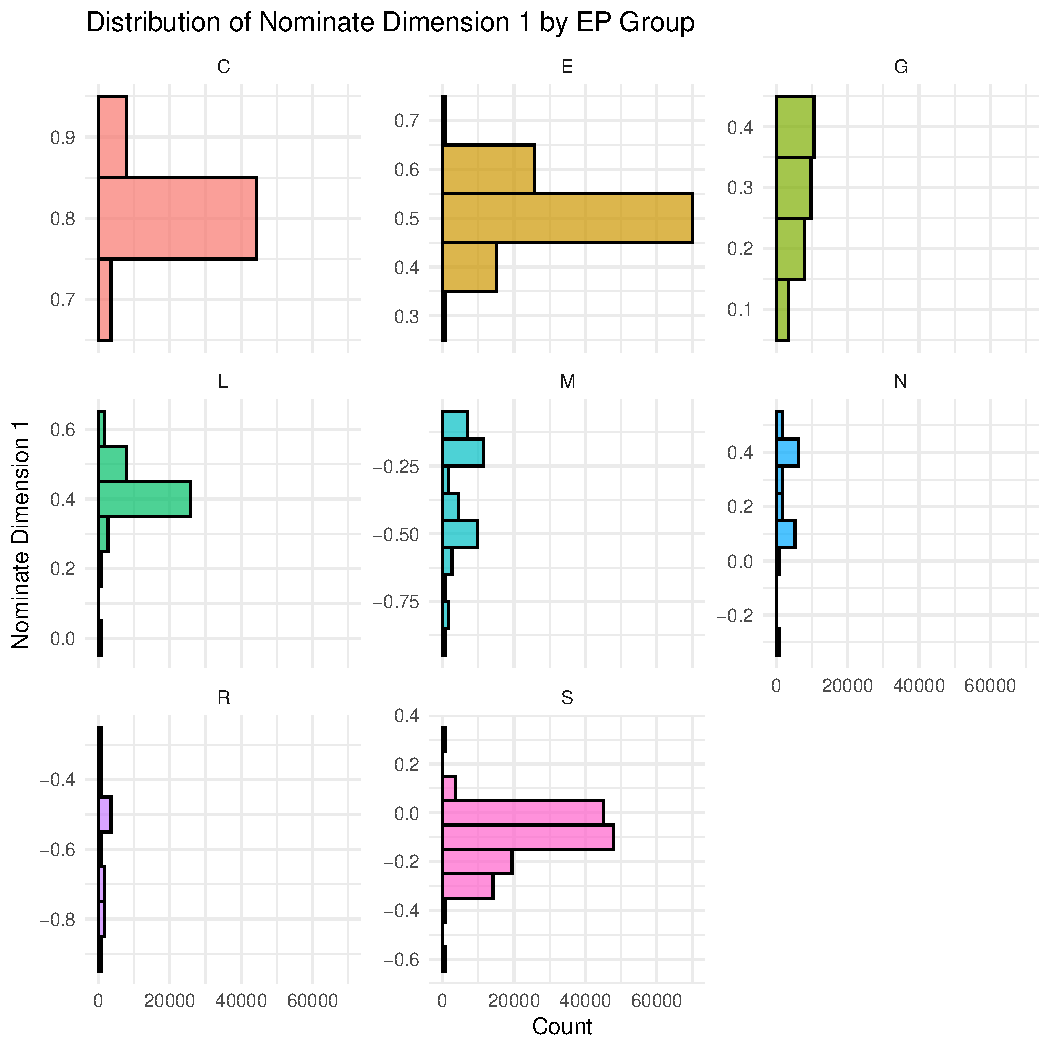
\includegraphics[width=0.7\textwidth]{Viz_1.pdf}
	\end{figure}
	\newpage
	\item Make a scatterplot of \textit{nomdim1} (x-axis) and \textit{nomdim2} (y-axis), with one point per MEP and color by EP group.  
	\begin{figure}[H]
		\centering
		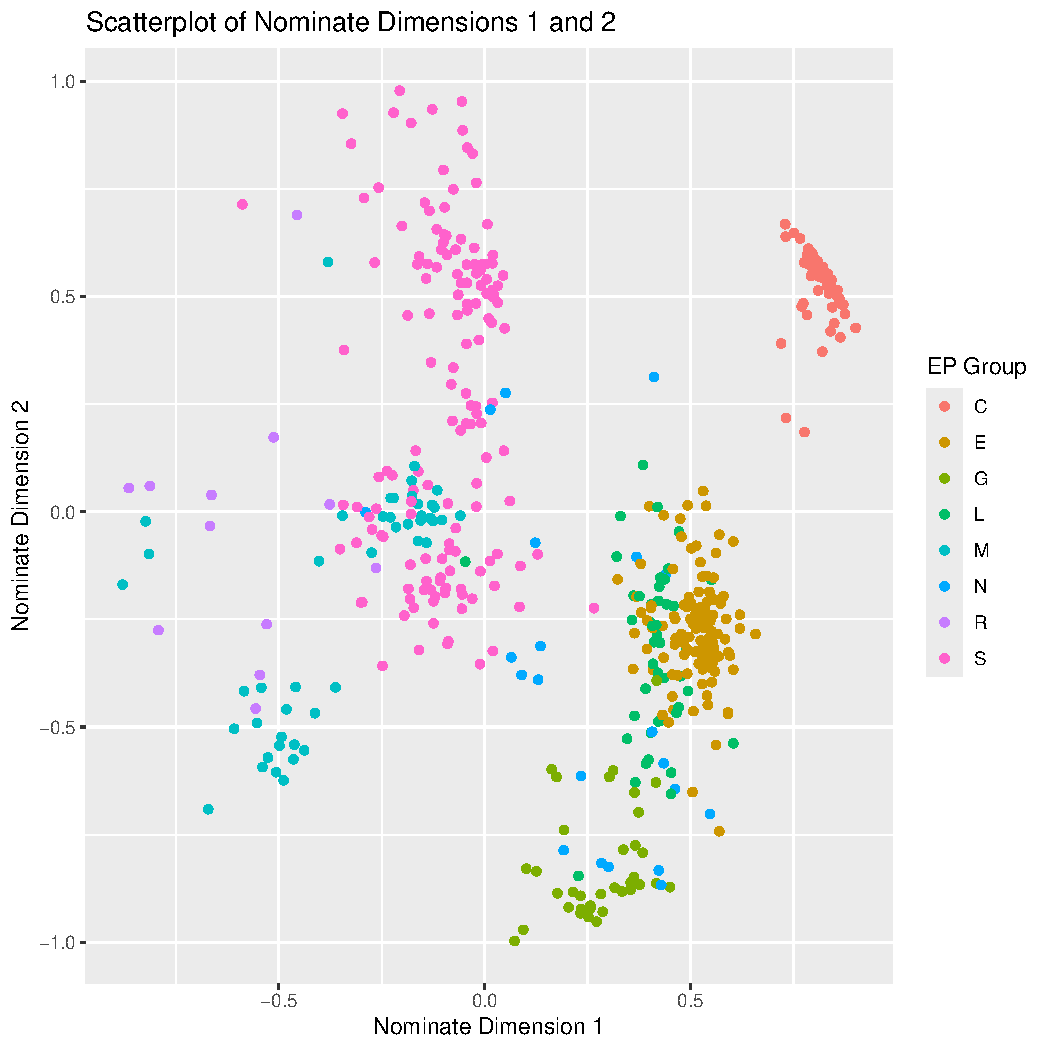
\includegraphics[width=0.7\textwidth]{Viz_2.pdf}
	\end{figure}
	\item Produce a boxplot of the proportion voting \textit{Yes} by EP group to visualize cohesion.  
	\begin{figure}[H]
		\centering
		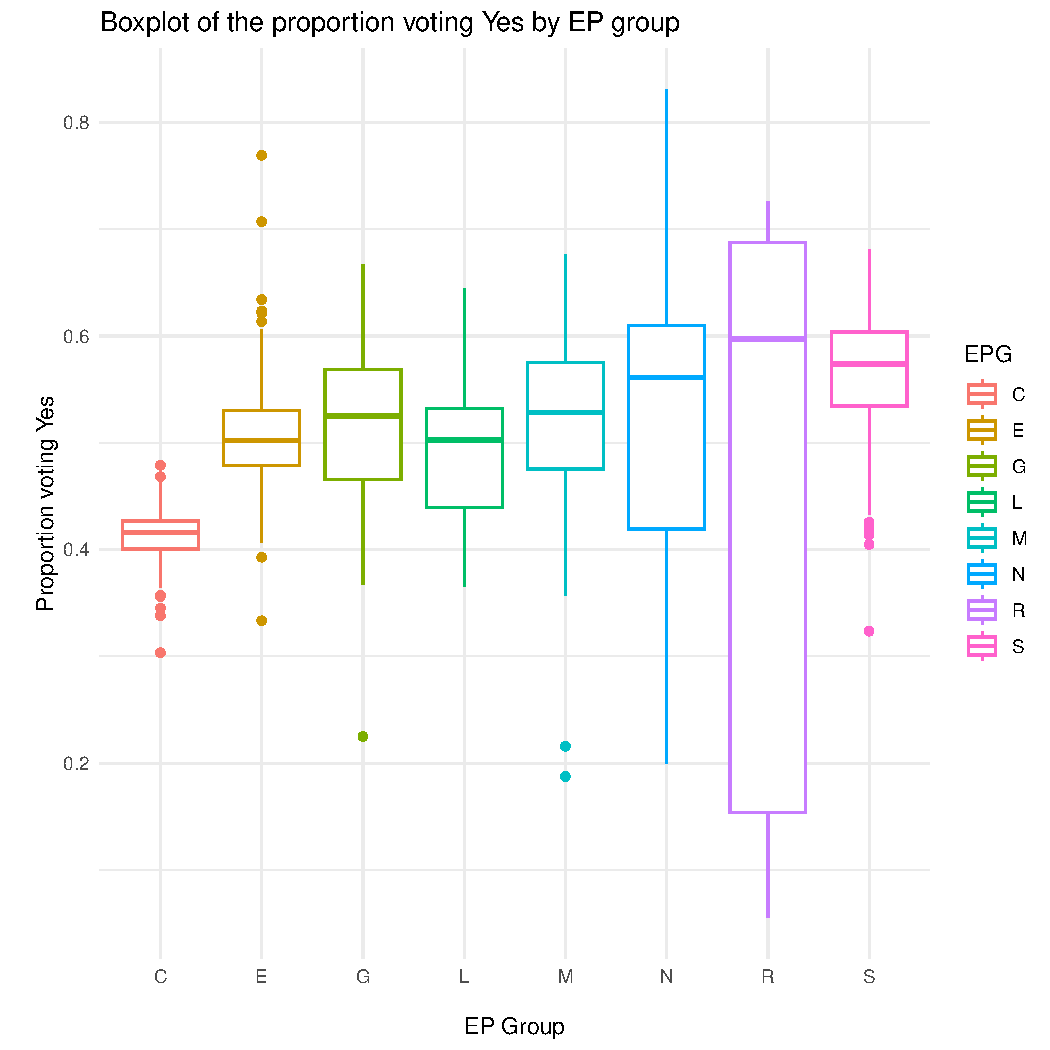
\includegraphics[width=0.7\textwidth]{Viz_3.pdf}
	\end{figure}
	\item Display the proportion voting \textit{Yes} per year by national party using a bar plot.  
	\begin{figure}[H]
		\centering
		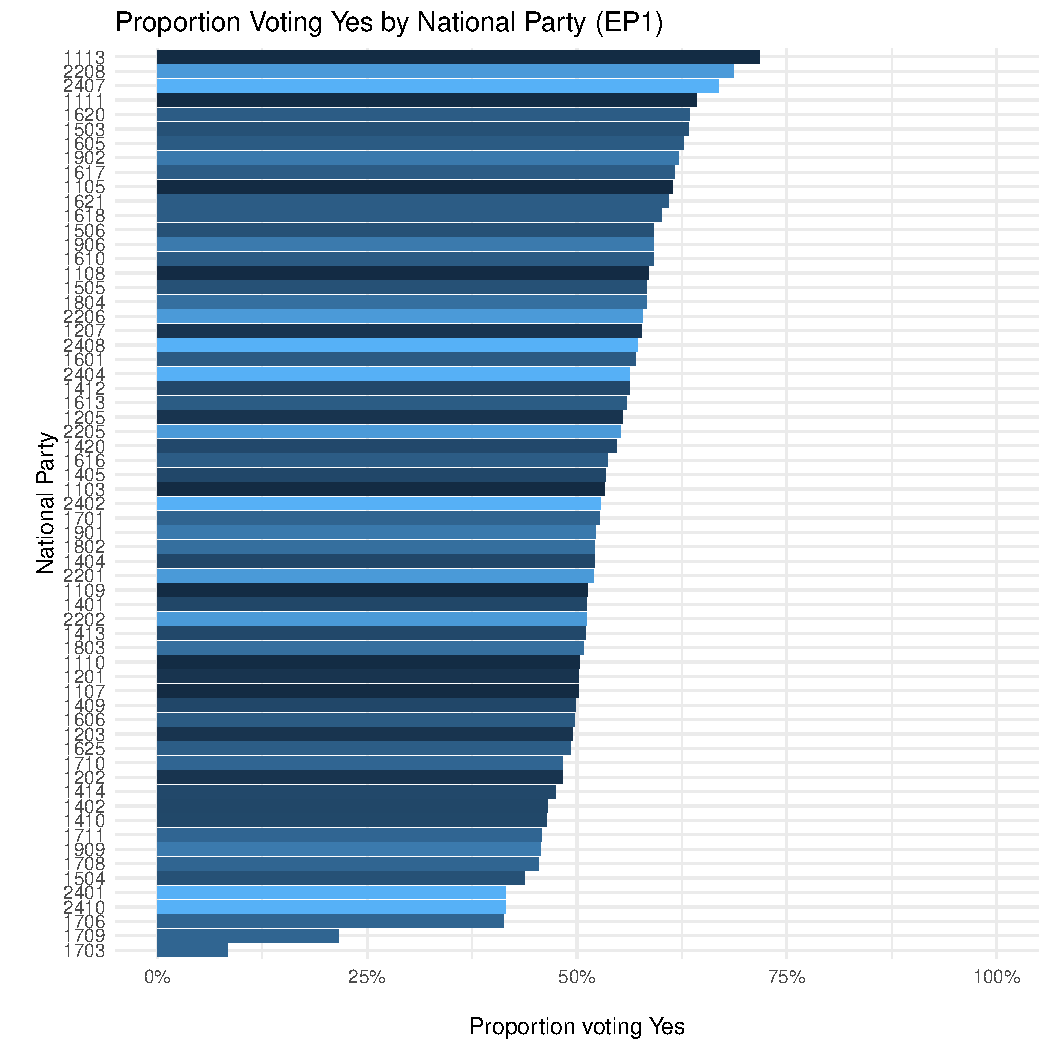
\includegraphics[width=0.7\textwidth]{Viz_4.pdf}
	\end{figure}
	\item For each EP group, calculate the average \textit{Yes} share per year and plot a line graph. 
	\begin{description}
		\item N/A
	\end{description}
\end{enumerate}



\end{document}
